\section{Prima valutazione sull'utilizzo di Android in contesti real-time}
Fin dalla sua nascita Android ha generato moltissimo interesse intorno a sé. Il fatto di essere open-source gli permette di essere ben studiato e compreso. Inoltre chiunque può provare a fare dei miglioramenti o ad adattarlo in base alle proprie esigenze. Ricercatori e non hanno provato a fondo le funzionalità offerte, portando e proponendo modifiche a vari livelli per scopi diversi: sicurezza, uso nell'industria, ecc. In molti hanno anche studiato la possibilità di utilizzarlo in contesti real-time. 

Tuttavia, Android non è stato pensato per un utilizzo in contesti con seri vincoli temporali. Molte scelte, architetturali e non, lo penalizzano in quest'ottica. Di seguito ne verranno analizzate alcune.

\subsection{Garbage Collection} \label{sec:gcandroid}
Il garbage collector di Android è di tipo stopping-the-world, e non può essere eseguito concorrentemente con l'applicazione. Inoltre, ogni applicazione in esecuzione ha un suo garbage collector. Infatti, in Android, ogni applicazione esegue utilizzando un'istanza della DVM. Un processo chiamato \textit{Zygote} viene avviato al boot e, a run-time, è responsabile di fare il fork della DVM. Fornisce inoltre un'area di memoria condivisa per tutte le applicazioni in esecuzione. Quest'area è disponibile per tutti i processi ed è mantenuta da Zygote. In più è presente un'area di memoria privata per ogni applicazione. I GC delle applicazioni possono eseguire concorrentemente l'un l'altro. I dati condivisi sono liberati dal GC di Zygote. Quando quest'ultimo è pronto per partire, per ragioni di consistenza, tutti i thread vengono fermati, e questo è un grande problema per le applicazioni real-time, perché l'applicazione è ferma mentre il runtime pulisce la memoria. La strategia di pulizia è di tipo mark-sweep, con tutti i vantaggi e gli svantaggi discussi nella Sezione~\ref{sec:gc}.

\subsection{Scheduler}
Android utilizza lo stesso algoritmo di scheduling del kernel Linux, ovvero \textbf{Completely Fair Scheduling} (CFS), un algoritmo basato sul concetto di virtual clock. Quest'ultimo misura la quantità di tempo di processore che, in un sistema completamente fair, sarebbe stata data ad un processo in attesa. Linux non memorizza questa informazione, ma la calcola a partire da una struttura simile alla seguente:
\begin{lstlisting}[language=c, caption={Entità schedulabile in Linux}, label={lst:schedentity}]
struct sched_entity {
	...
	u64 exec_start;
	u64 sum_exec_runtime;
	u64 vruntime;
	u64 prev_sum_exec_runtime;
	...
}
\end{lstlisting}
Quando un processo è assegnato ad una CPU, \texttt{exec\_start} è aggiornato all'istante attuale e il tempo di esecuzione è memorizzato in \texttt{sum\_exec\_runtime}. Quando il processo lascia la CPU \texttt{sum\_exec\_runtime} viene copiato in \texttt{prev\_sum\_exec\_runtime}. \texttt{sum\_exec\_runtime} è calcolato incrementalmente, cioè cresce monotonicamente. Infine, \texttt{vruntime} memorizza l'ammontare di tempo che è trascorso nel virtual clock durante l'esecuzione del processo. Quest'ultimo è incrementato della seguente quantità:
\[ delta\_exec\_weighted = delta\_exec * \frac{NICE\_0\_LOAD}{load\_weight}; \]
dove \texttt{delta\_exec} è il tempo di CPU del processo e \texttt{load\_weight} è il peso del processo. L'utilizzo a denominatore del peso può essere considerato come un fattore di correzione. Task con alta priorità (e con basso valore nice) avranno peso maggiore. Di conseguenza l'incremento di \texttt{vruntime} sarà piccolo. Run-time virtuale e fisico sono uguali per task con $nice = 0$ e priorità 120, cioè quando $load\_weight = NICE\_0\_LOAD$. Solitamente un aumento di nice di 1 unità risulta in un tempo di CPU minore di circa 10\%. 

La coda di esecuzione è mantenuta in un albero rosso nero e ogni coda (una per CPU) memorizza un campo \texttt{min\_vruntime}. Quest'ultimo rappresenta il più piccolo \texttt{vruntime} tra tutti i processi nella coda (di conseguenza può solo aumentare, e mai diminuire). Le chiavi per i nodi dell'albero rosso nero sono date da $vruntime - min\_vruntime$, per ogni processo nella coda.

Quando lo scheduler è invocato, il kernel prende il task con la chiave minore (che sarà memorizzato nella posizione più a sinistra), e gli assegna la CPU. Quindi gli elementi con chiave minore sono posizionati più a sinistra, e saranno eseguiti prima.

Quando un processo esegue, il suo \texttt{vruntime} aumenta costantemente, fino a quando non si posizionerà nella parte più a destra dell'albero. Dato che questo campo aumenta più lentamente per i task ad alta priorità, loro si muoveranno verso destra più lentamente. Questo significa che loro hanno più possibilità di essere eseguiti rispetto a quelli a bassa priorità, come è giusto che sia. Se un processo è in attesa il suo \texttt{vruntime} resta inalterato, ma dato che il \texttt{min\_vruntime} della cosa aumenta costantemente prima o poi quel processo verrà svegliato perché la sua chiave è diventata la minore. 

In questo protocollo non ci sono possibilità di starvation, dato che prima o poi tutti verranno eseguiti. Inoltre, se un task si mette in attesa per I/O verrà ricompensato con tutta la quantità di tempo che è stata necessaria per completare l'operazione. 

Lo scheduler di Linux è modulare e prevede diverse classi di scheduling per poter utilizzare diversi algoritmi/politiche per diverse occasioni. Una classe di scheduling di fatto fornisce un'interfaccia allo scheduler principale per permettere di gestire task usando diversi algoritmi. Come previsto dallo standard POSIX, Linux dispone di due classi soft real-time: \textbf{SCHED\_RR}, per politiche round robin, e \textbf{SCHED\_FIFO}, per politiche FIFO. Android però fa scheduling utilizzando prevalentemente \textbf{SCHED\_OTHER}, che non offre nessun supporto real-time.

Di conseguenza lo scheduling di Android da più importanza alla fairness, una proprietà che non interessa ai sistemi real-time. 

\subsection{Gestione di interruzioni ed eventi}
Il kernel è responsabile di notificare l'applicazione quando arriva un'interruzione o si verifica un evento. Purtroppo però nessuna componente coinvolta in questo meccanismo ha la nozione di restrizioni temporali. Inoltre in Linux le interruzioni sono task con la massima priorità. Quindi un task in esecuzione ad alta priorità (ma non massima) può essere prerilasciato dall'arrivo di una interruzione. A causa di questo grande problema il sistema non può essere considerato completamente prevedibile.

\subsection{Framework applicativo}
\subsubsection{Costrutti e API}
Tra tutti i componenti forniti da Android, \texttt{Looper} e \texttt{Handler} sono i più problematici e pervasivi. Anche se un'applicazione non li usa esplicitamente, questi vengono implicitamente utilizzati dal runtime per controllarne il flusso, in particolare le transizioni tra gli stati di una Activity. Il problema principale è che la latenza della consegna dei messaggi a questi componenti non è prevedibile: thread con bassa priorità possono impedire a thread con priorità più alta di eseguire, senza motivo. 

\begin{figure}[h]
	\centering
	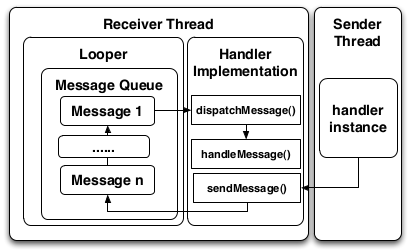
\includegraphics[width=0.5\linewidth]{looperHandler}
	\caption{Utilizzo di \texttt{Looper} e \texttt{Handler}}
	\label{fig:looperhandler}
\end{figure}
Figura~\ref{fig:looperhandler} mostra il funzionamento dei due costrutti. \texttt{Looper} si occupa di mantenere in un thread una coda di messaggi e di inviarli all'\texttt{Handler} opportuno, che li processerà. Il programmatore fornisce la logica per processare il messaggio implementando il metodo \texttt{handleMessage()} di \texttt{Handler}. Un'istanza di \texttt{Handler} è condivisa tra due thread per inviare e ricevere messaggi. Questo meccanismo è problematico quando più thread a priorità diverse inviano messaggi contemporaneamente. Ci sono due modi in cui i messaggi vengono processati. Di default l'ordine seguito è quello di ricezione. In aggiunta, però, un mittente può specificare un istante temporale nel quale il messaggio dovrà essere processato. In entrambi i casi però non viene considerata la priorità dei thread coinvolti. Se molti thread non real-time inviano simultaneamente messaggi allo stesso thread, insieme ad uno real-time, i messaggi di quest'ultimo saranno considerati solo dopo tutti i messaggi precedenti (Figura~\ref{fig:looperhandlerissue}). Inoltre, se altri thread non real-time inviano messaggi specificando un istante per processarli, la coda viene riordinata a run-time per fare in modo che questi messaggi vengano considerati in quel preciso istante. Questo significa che un thread real-time ad alta priorità può vedersi passare avanti un sacco di messaggi inviati da altri thread con una priorità molto più bassa.
\begin{figure}
	\centering
	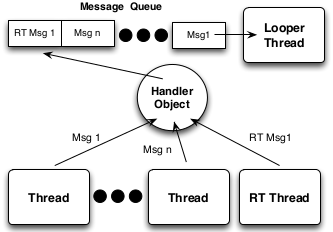
\includegraphics[width=0.5\linewidth]{looperHandlerissue}
	\caption{Scenario di ritardo per un thread real-time}
	\label{fig:looperhandlerissue}
\end{figure}

\subsubsection{Servizi di sistema}
L'implementazione di servizi come \texttt{SensorManager} o \texttt{AlarmManager}, utilizzati fortemente in applicazioni per il sensing dell'ambiente circostante, non tengono conto di eventuali vincoli temporali. 

\paragraph{AlarmManager.} Un'applicazione che vuole impostare un allarme invia un messaggio ad \texttt{AlarmManager}. Quando l'allarme scatta, all'istante specificato dall'applicazione, questa viene notificata e un metodo di callback, definito all'invio del primo messaggio, viene eseguito. Il problema è che non viene data nessuna garanzia sul tempo trascorso dallo scattare dell'allarme al momento in cui l'applicazione ne viene a conoscenza. 

\paragraph{SensorManager.}
Un'applicazione può ascoltare l'ambiente circostante attraverso le API di \texttt{SensorManager} e fornire delle callback. Queste vengono chiamate ogni volta che un evento di interesse si verifica. Ci sono due principali problemi: 
\begin{itemize}
	\item non c'è nessun supporto per le priorità dei thread, dato che tutti gli eventi finiscono nella stessa coda. Un thread ad alta priorità può dover aspettare un sacco di thread a priorità minore prima di ricevere i dati di cui ha bisogno;
	\item la consegna degli eventi avviene tramite uno scambio di messaggi tra tutte le classi coinvolte nel sensing. Android non fornisce nessuna garanzia sul tempo necessario a consegnare questi messaggi.
\end{itemize}

\subsection{Fonti di Jitter}
Figura~\ref{fig:androidjitter} mostra una tassonomia delle fonti di jitter in Android. 
\begin{figure}[h]
	\centering
	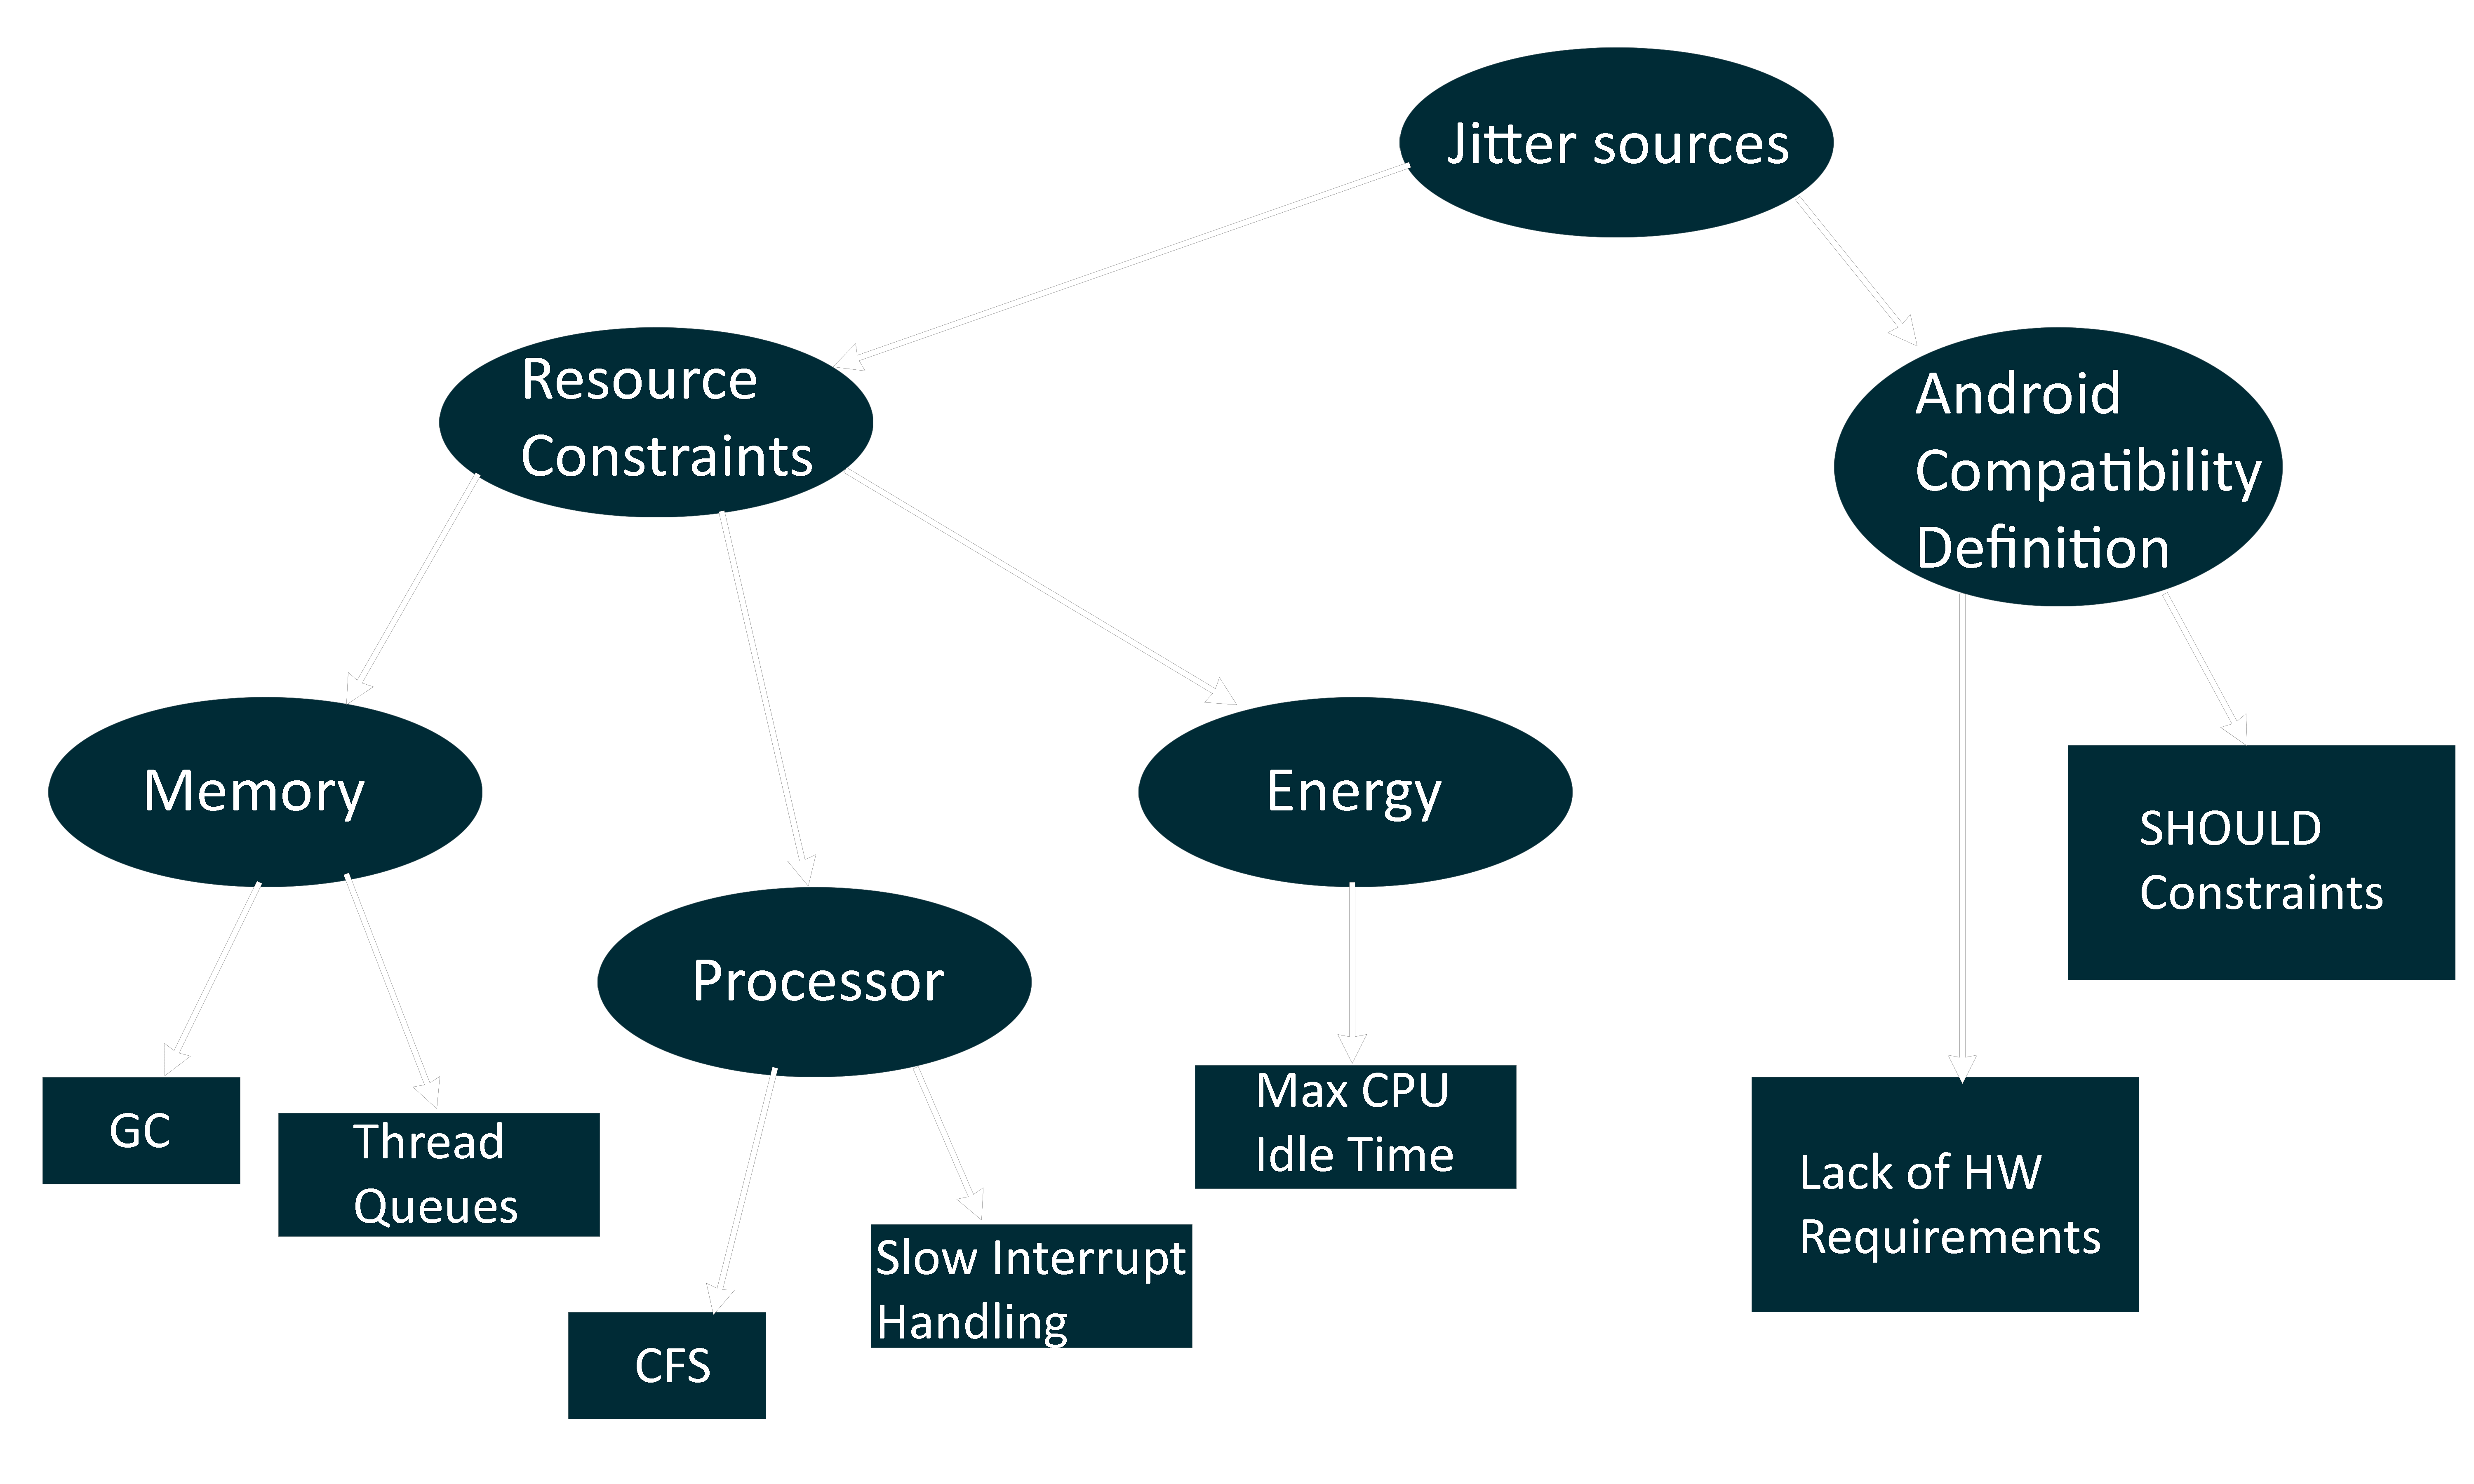
\includegraphics[width=1\linewidth]{androidJitter}
	\caption{Tassonomia delle fonti di jitter in Android}
	\label{fig:androidjitter}
\end{figure}

Android è jitter-prone per definizione e necessità. I primi requisiti sul jitter sono stati imposti a partire da CDD 5.0 (Android Compatibility Definition Document, un documento che specifica i requisiti delle implementazioni di Android), e anche in quello sono indicati come SHOULD (cioè raccomandati, ma non obbligatori). In aggiunta, i dispositivi Android hanno risorse limitate (e sono molto eterogenei). Di conseguenza, la gestione al risparmio di memoria, CPU ed energia è in contrasto con l'acquisizione accurata di dati dai sensori.

\paragraph{Concorrenza} \mbox{} \\
I ritardi collegati alla concorrenza sono legati alla latenza introdotta da multiple entità schedulabili che competono per l'esecuzione. Il fatto che molti componenti Android possono essere soggetti a ritardi non limitati è un serio problema per le applicazioni real-time. Come già visto, Android si basa su CFS che, per minimizzare la unfairness, può permettere a task a bassa priorità di eseguire al posto di altri ad alta priorità, causando così il fenomeno di priority inversion. Inoltre, dato che viene utilizzato un albero rosso nero, le operazioni di inserimento e rimozione dalla ''coda'' chiedono un tempo $O(log(n))$, dove \textit{n} è il numero di entità in competizione. Infine, sebbene la libreria standard di C preveda meccanismi per prevenire l'inversione di priorità, l'implementazione di Android, Bionic, non li prevede. Di conseguenza lo scheduling può essere problematico se la congestione è alta.

\paragraph{Vincoli di memoria} \mbox{} \\
Viste le limitate quantità di memoria di alcuni dispositivi Android, il sistema cerca di liberarla il più spesso possibile. Di conseguenza la garbage collection è molto aggressiva. Inoltre, in condizioni critiche, la coda dei pronti non può essere memorizzata in RAM, e deve essere salvata nella memoria secondaria, causando ritardi altissimi.

\paragraph{Risparmio energetico} \mbox{} \\
Per risparmiare la batteria Android cerca di sospendere le CPU il più spesso possibile. Le transizioni da sleep a wake sono estremamente lente, e causano jitter molto elevati. Inoltre Android privilegia il risparmio energetico all'accuratezza delle misurazioni. Infatti, uno dei requisiti di \texttt{SensorManager} è ''MUST NOT prevent the device CPU from entering a suspend state or waking up from a suspend state''.